\subsection{Mission Breakdown}
\label{sec:flightmaneuvers}
The Medical Express mission can be broken down into three distinct flight maneuvers:
\begin{enumerate}[label=\bfseries M\arabic*:] \itemsep-2pt
	\item Hover flight, including vertical take-off to cruising height, and landing
	\item Fixed-wing flight, navigating through waypoints and keeping within GeoFence boundaries
	\item Aerial search of target area to find Joe
\end{enumerate}

Using these maneuvers, completing the mission can be described as completing the sequence of actions\\
\begin{tabular}{r l l}
	1. & Mission start after being armed & (\textbf{M1}) \\ 
	2. & Navigate to Joe's location & (\textbf{M2}) \\ 
	3. & Aerial search to identify Joe & (\textbf{M3}) \\ 
	4. & Land near Joe to collect blood & (\textbf{M1}) \\ 
	5. & Take-off after being re-armed & (\textbf{M1}) \\ 
	6. & Navigate back to base & (\textbf{M2}) \\ 
	7. & Land at base & (\textbf{M1}) \\ 
\end{tabular}\\

Executing this mission on a purely fixed-wing or rotor-based aircraft is unlikely to be successful; instead, teams will need to design an aircraft that makes use of both flight modes. Analysis of the aircraft developed by the 2014 team (see Appendix \ref{sec:lastYear} for full details) showed that converting the purely fixed-wing aircraft to a hybrid would not result in a design capable of competing in the UAV Challenge. Given the aircraft's weight, fitting it with flight equipment (motors, supports, power) to provide VTOL capabilities would add over 5kg, cost over \$500, and would result in less than 60 seconds of flight time. It was therefore decided the 2014 model would not be suitable for the 2016 competition, and several alternative solutions were investigated.\\

As this project involves the development of a novel UAV platform, there is a lack of academic literature that is relevant to the problem at hand. This review will instead collate examples of commercial and hobby systems that were used to motivate the design of the UAV developed in this project.\\

\subsection{Aircraft Design}
\label{sec:litaircraft}
\subsubsection*{Arcturus Jump}
The Arcturus Jump \cite{ref:arcturus} (Figure \ref{fig:arcturus}) is a quad-copter/fixed-wing hybrid, with propellers mounted across the wings for VTOL, and a propeller at on the nose for fixed-wing flight. Modifying an existing airframe to emulate this design would be straightforward, but the addition of the support structure for VTOL flight would add significant weight to the aircraft, decreasing thrust and maneuverability, as well as increasing drag. These factors make an aircraft of this design unlikely to achieve requirements \textbf{R3} and \textbf{R4} of the UAV Challenge.

\begin{figure}[!h]
	\centering
	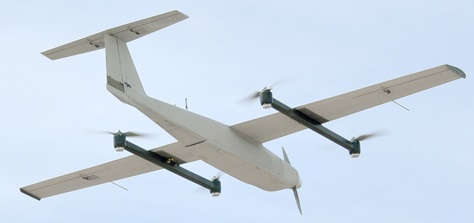
\includegraphics[width=150pt]{\IMAGEPATH /Aircraft/arcturus}
	\caption{Jump 20, by Arcturus}
	\label{fig:arcturus}
\end{figure}

\subsubsection*{X PlusOne}
The X PlusOne \cite{ref:xplusone} (Figure \ref{fig:xplusone}) is a fast and efficient hybrid with four front-facing propellers, enabling it to fly in both VTOL and fixed-wing modes. It is extremely small and light, but does not have the range and endurance capabilities required. A UAV of this form would be relatively cheap to build, but is too small to replicate with an existing airframe. Based on the activities of the 2014 UAV team, designing a completely new airframe would take a significant amount of time, and is not advised for this project.

\begin{figure}[!ht]
	\centering
	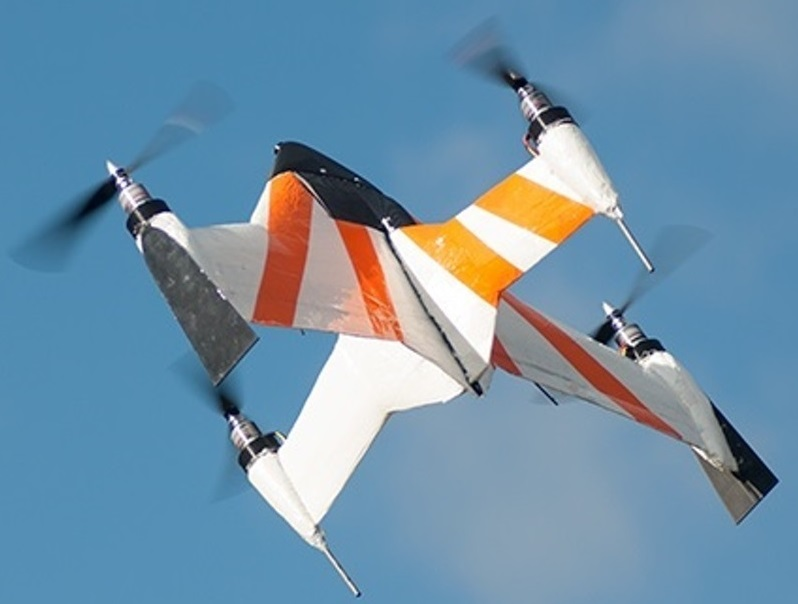
\includegraphics[width=120pt]{\IMAGEPATH /Aircraft/xplusone}
	\caption{X PlusOne, by XCraft}
	\label{fig:xplusone}
\end{figure}

\subsubsection*{TBS Caipirinha}
The TBS Caipirinha \cite{ref:caipirinha} (Figure \ref{fig:caipirinha}) is traditionally a hobbyist fixed-wing aircraft kit. However, several examples have shown it is possible to modify the Caipirinha to be a VTOL aircraft \cite{ref:caipirinhaVTOL} (Figure \ref{fig:caipirinhaVTOL}), with two front-facing propellers. Modifying the Caipirinha for hybrid flight would require minimal modifications to the airframe, but would require the development of advanced control systems to alternate between VTOL and fixed-wing modes.

\begin{figure}[!ht]
	\centering
	\begin{minipage}{.5\textwidth}
		\centering
		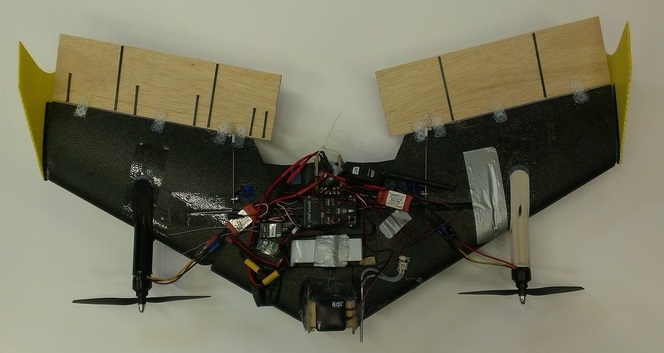
\includegraphics[width=135pt]{\IMAGEPATH /Aircraft/caipirinha}
		\caption{TBS Caipirinha, by Mongrel Gear}
		\label{fig:caipirinha}
	\end{minipage}%
	\begin{minipage}{.5\textwidth}
		\centering
		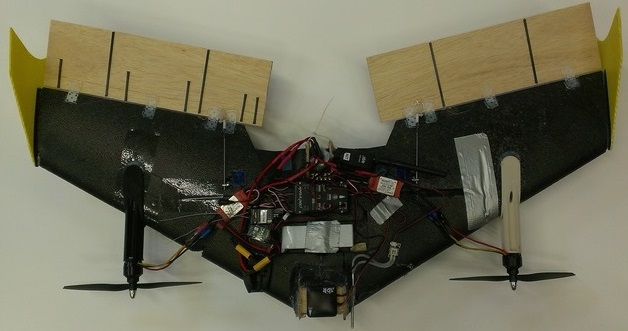
\includegraphics[width=155pt]{\IMAGEPATH /Aircraft/caipirinhaVTOL}
		\caption{Caipirinha modified by PX4 for VTOL flight}
		\label{fig:caipirinhaVTOL}
	\end{minipage}
\end{figure}

\subsubsection*{Aerosense AS-DT01-E}
The Aerosense AS-DT01-E \cite{ref:sony} (Figure \ref{fig:sony}) is an autonomous hybrid VTOL/fixed-wing aircraft under development by Sony Mobile in partnership with Japanese company ZMP. While the prototype aircraft would be an ideal candidate for the Challenge, as with the X PlusOne, the design and construction of the airframe would be time consuming, and is not advised for this project.

\begin{figure}[!ht]
	\centering
	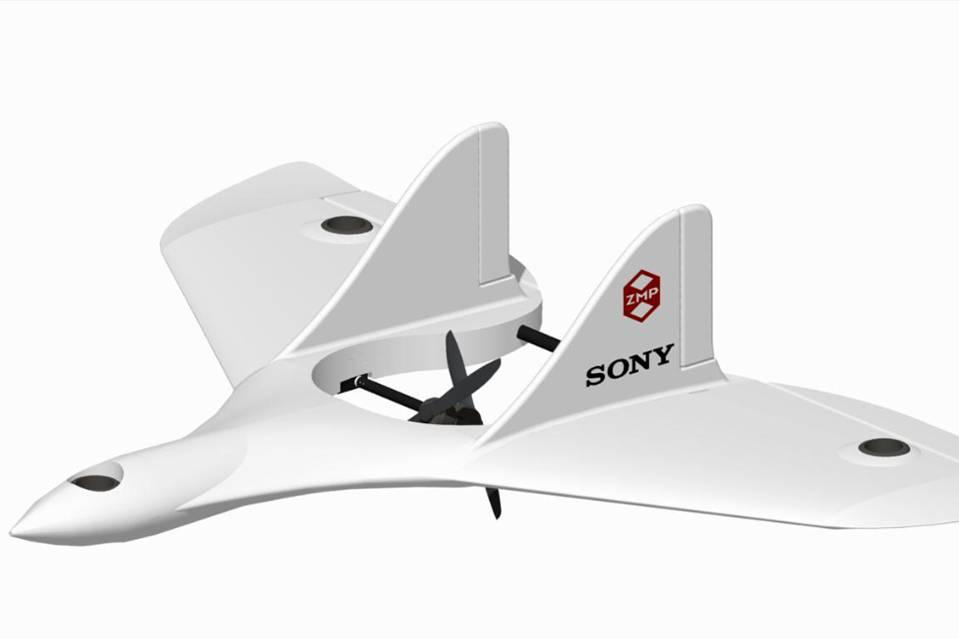
\includegraphics[width=160pt]{\IMAGEPATH /Aircraft/sony}
	\caption{Aerosense AS-DT01-E, by Sony and ZMP}
	\label{fig:sony}
\end{figure}

\subsubsection*{FireFLY6}
The FireFLY6 \cite{ref:firefly6} (Figure \ref{fig:firefly6}) is a remote control hybrid VTOL/fixed-wing aircraft consisting of six propellers arranged in 3 sets of two (Y-6 configuration). This design can achieve 20-30 minutes of flight time, seven minutes of hover, and a cruising speed of 54km/h, and with modification would be a strong contender in the UAV Challenge.

\begin{figure}[!h]
	\centering
	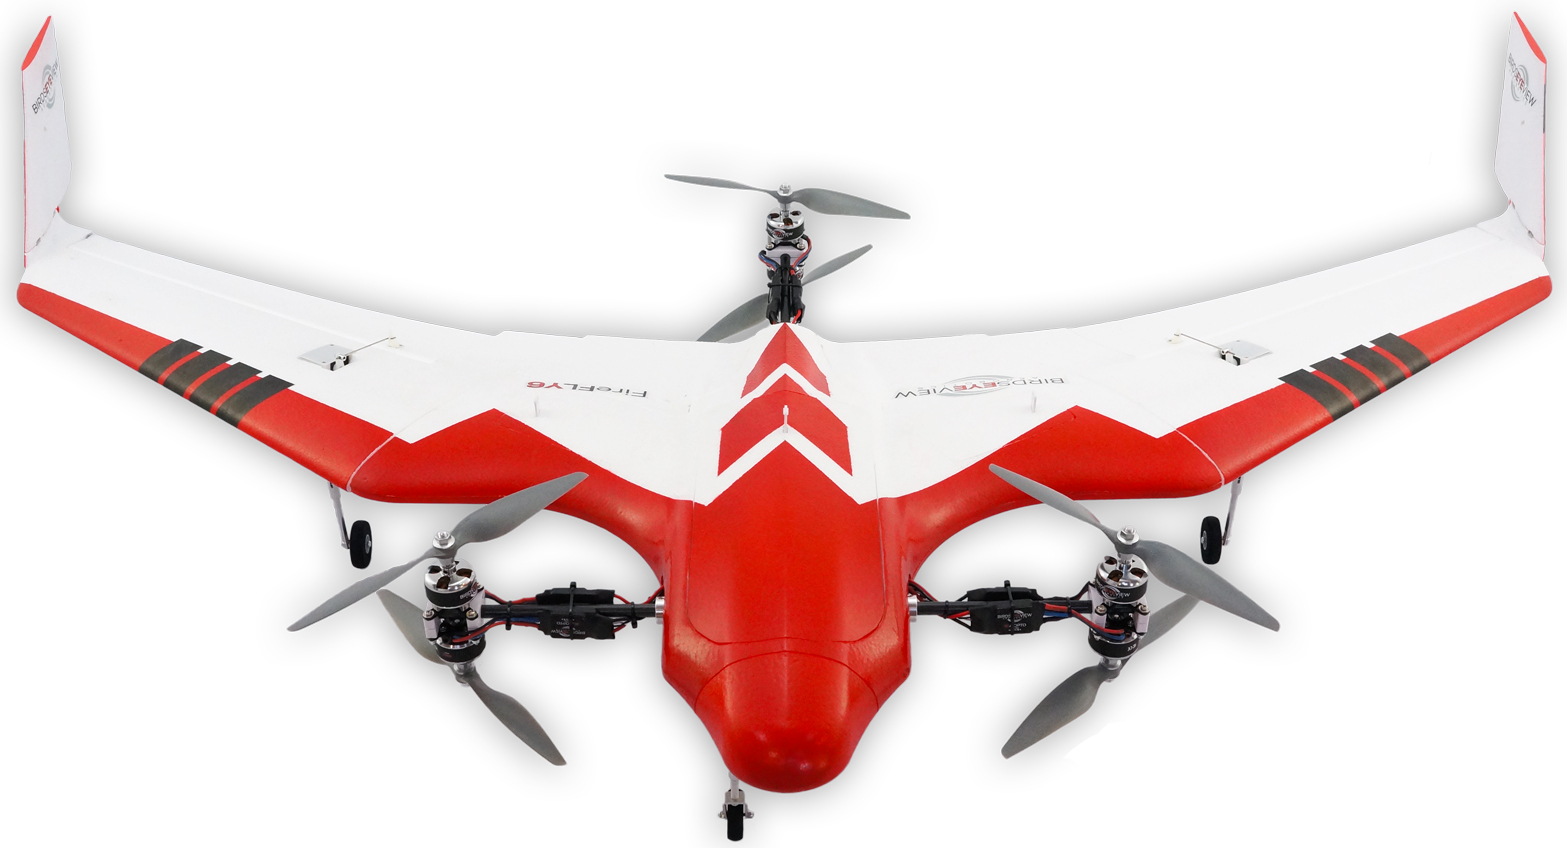
\includegraphics[width=160pt]{\IMAGEPATH /Aircraft/firefly6}
	\caption{FireFLY6, by BirdsEyeView Aerobotics}
	\label{fig:firefly6}
\end{figure}